\documentclass[10pt]{beamer}
\usetheme[
%%% options passed to the outer theme
%    hidetitle,           % hide the (short) title in the sidebar
%    hideauthor,          % hide the (short) author in the sidebar
%    hideinstitute,       % hide the (short) institute in the bottom of the sidebar
%    shownavsym,          % show the navigation symbols
%    width=2cm,           % width of the sidebar (default is 2 cm)
%    hideothersubsections,% hide all subsections but the subsections in the current section
%    hideallsubsections,  % hide all subsections
%    left                % right of left position of sidebar (default is right)
]{Aalborg}
  
% If you want to change the colors of the various elements in the theme, edit and uncomment the following lines
% Change the bar and sidebar colors:
%\setbeamercolor{Aalborg}{fg=red!20,bg=red}
%\setbeamercolor{sidebar}{bg=red!20}
% Change the color of the structural elements:
%\setbeamercolor{structure}{fg=red}
% Change the frame title text color:
%\setbeamercolor{frametitle}{fg=blue}
% Change the normal text color background:
%\setbeamercolor{normal text}{bg=gray!10}
% ... and you can of course change a lot more - see the beamer user manual.
\usepackage[utf8]{inputenc}
\usepackage[brazil]{babel}
\usepackage[T1]{fontenc}
% Or whatever. Note that the encoding and the font should match. If T1
% does not look nice, try deleting the line with the fontenc.
\usepackage{helvet}
\usepackage{animate}

\usepackage{xcolor}
% Definindo cores
\definecolor{beaublue}{rgb}{0.74, 0.83, 0.9}
\definecolor{softgray}{rgb}{0.9, 0.9, 0.9}

% colored hyperlinks
\newcommand{\chref}[2]{%
  \href{#1}{{\usebeamercolor[bg]{Aalborg}#2}}%
}

\title[Minicurso Docker]% optional, use only with long paper titles
{\huge
\textbf{Minicurso Docker}
}

%\subtitle{Jogo da Velocidade}  % could also be a conference name

\date{\today}

\author[Gian Lucas] % optional, use only with lots of authors
{
  Gian Lucas Cavalcante de Lima
}
% - Give the names in the same order as they appear in the paper.
% - Use the \inst{?} command only if the authors have different
%   affiliation. See the beamer manual for an example

\institute[
%  {\includegraphics[scale=0.2]{aau_segl}}\\ %insert a company, department or university logo
  Lógica Sistemas\\ LTDA
] % optional - is placed in the bottom of the sidebar on every slide
{ % is placed on the bottom of the title page
  Lógica Sistemas de Informação
  
  %there must be an empty line above this line - otherwise some unwanted space is added between the university and the country (I do not know why;( )
}

% specify the logo in the top right/left of the slide
\pgfdeclareimage[height=0.8cm]{mainlogo}{AAUgraphics/logo} % placed in the upper left/right corner
\logo{\pgfuseimage{mainlogo}}

% specify a logo on the titlepage (you can specify additional logos an include them in 
% institute command below
\pgfdeclareimage[height=1.6cm]{titlepagelogo}{AAUgraphics/logo} % placed on the title page
%\pgfdeclareimage[height=1.5cm]{titlepagelogo2}{AAUgraphics/aau_logo_new} % placed on the title page
\titlegraphic{% is placed on the bottom of the title page
  \pgfuseimage{titlepagelogo}
%  \hspace{1cm}\pgfuseimage{titlepagelogo2}
}
% Colocar gif
% https://tex.stackexchange.com/questions/240243/getting-gif-and-or-moving-images-into-a-latex-presentation

\begin{document}
% the titlepage
{\aauwavesbg
\begin{frame}[plain,noframenumbering] % the plain option removes the sidebar and header from the title page
  \titlepage
\end{frame}
}
%%%%%%%%%%%%%%%%
% TOC
%\begin{frame}{Sumário}{}
%\tableofcontents
%\end{frame}

% \\\\\\\\\\\\\\\\\\\\\\\\\\\\\\\\\\\\\\\\\\\\\\\\\\\\\\\\
%  )||||||||||||||||||| CONCEITOS ||||||||||||||||||||||||)
% ////////////////////////////////////////////////////////
\section{Introdução}

\subsection{O que é Docker?}
\begin{frame}{Introdução}{}
    \begin{block}{\textbf{O que é Docker?}}
        Docker é uma plataforma de código aberto, escrito em Go e criado pela Google, para facilitar os processos de desenvolvimento e implantação de uma aplicação.
        \begin{itemize}
            \item<2-> O que o Docker faz é criar um ambiente sandbox, isolado do resto do sistema aonde uma aplicação vai rodar.
            \item<3-> Chamado \textit{Container}.
            %\item<4-> 
        \end{itemize}
    \end{block}
\end{frame}

\subsection{O que é um Container?}
\begin{frame}{O que é Docker?}{Introdução}
    \begin{block}{\textbf{Como funciona?}}
        Uma aplicação é encapsulada com suas dependências dentro de um container, aonde ela irá rodar isolada do resto do sistema. 
        \begin{itemize}
            \item<2-> não corre risco de sofrer interferências do meio externo.
            \item<3-> Similar a uma máquina virtual.
        \end{itemize}
    \end{block}
\end{frame}

\subsection{Container vs VM}
\begin{frame}{Container vs VM}{Introdução}
    \begin{block}{\textbf{Então Container é uma Máquina Virtual?}}
        \pause
        Containers não são máquinas virtuais, porém ambos possuam o mesmo objetivo.
    \end{block}
    \pause
    \begin{block}{\textbf{Qual a diferença?}}
        A principal diferença entre eles esta na sua arquitetura.
        \begin{itemize}
            \item<4-> Numa Máquina Virtual é feita a emulação de toda uma máquina guest, desde o software ao hardware, em cima de uma máquina host.
            \item<5-> Para fazer isso as VMs usam de um artifício chamado de Hypervisor.
            \item<6-> O Hypervisor é uma camada que fica entre o SO do Host e a máquina guest, e é ela que é responsável por fazer o intermédio entre os dois sistemas.
        \end{itemize}
    \end{block}
\end{frame}
\begin{frame}{Container vs VM}{Introdução}
    \begin{columns}
    \begin{column}{0.5\textwidth}
        \centering
        \textbf{Camadas VM}\\
        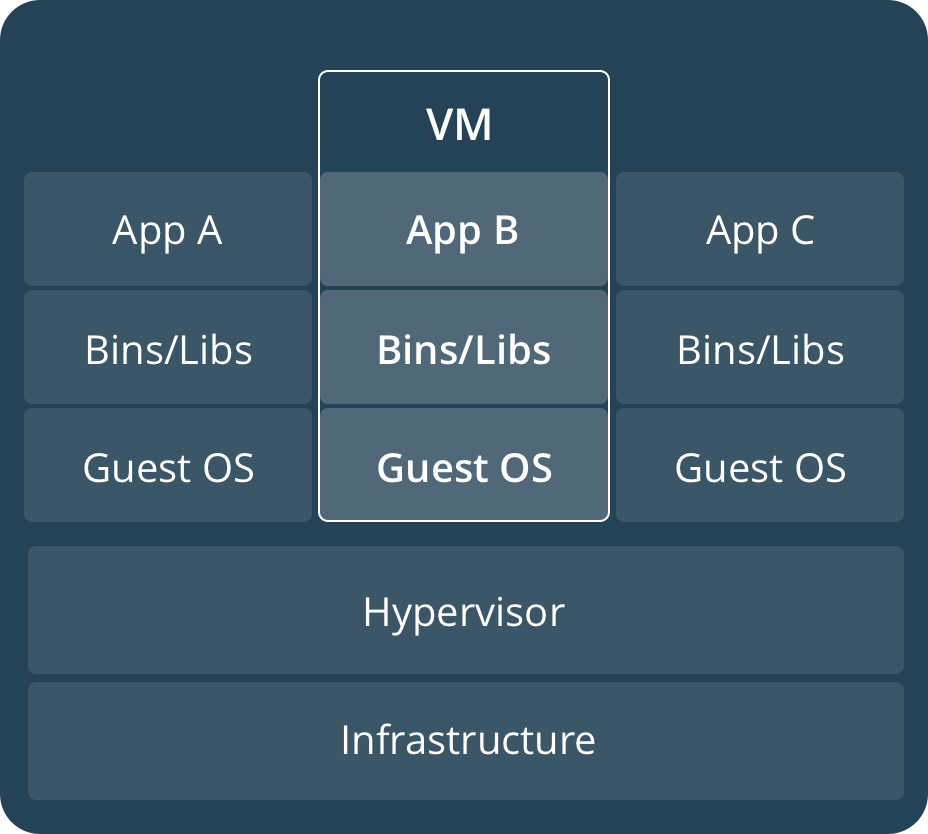
\includegraphics[width=0.75\textwidth]{AAUgraphics/camadas_vm.png}
    \end{column}
    \begin{column}{0.5\textwidth}  %%<--- here
        \centering
        \textbf{Camadas Container}\\
        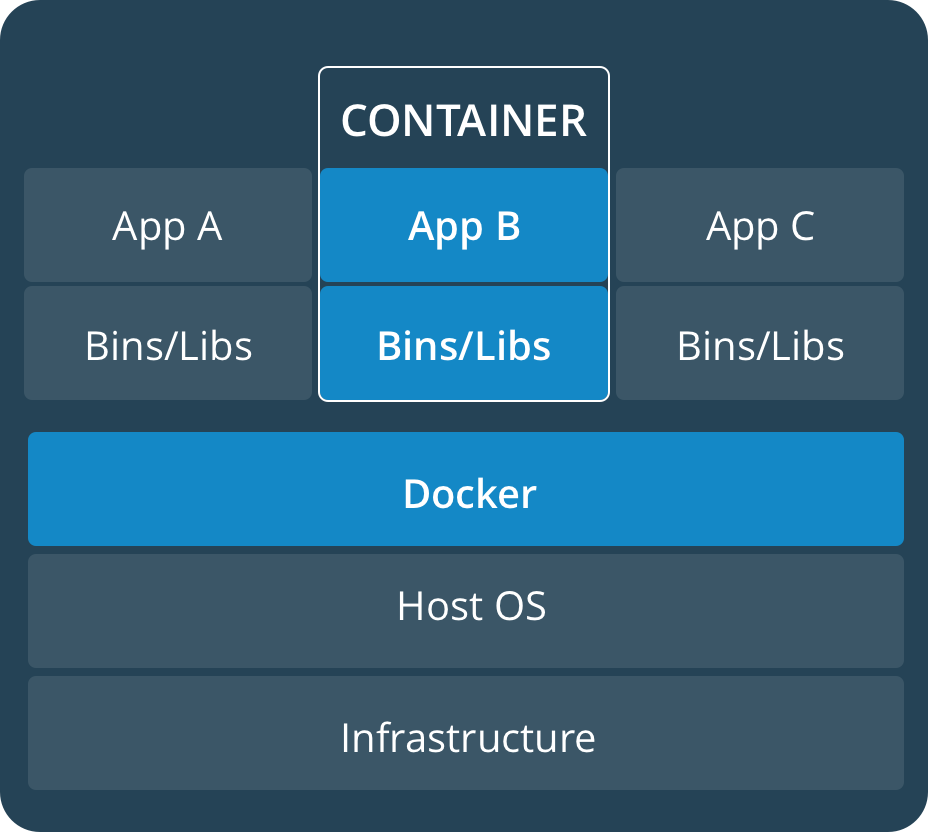
\includegraphics[width=0.75\textwidth]{AAUgraphics/camadas_container.png}
    \end{column}
    \end{columns}
\end{frame}

\subsection{Por que Docker?}
\begin{frame}{Por que Docker?}{Introdução}
    \begin{block}{\textbf{Facilidade}} 
        Docker foi criado de forma a ser fácil de usar, tendo em vista que desenvolvedores, administradores de sistemas, e outros usuários possam tomar vantagem de containers para rapidamente construir e testar aplicações. Ele permite que qualquer um possa empacotar uma aplicação no seu computador e possa move-lo para outra máquina ou plataforma.
    \end{block}
\end{frame}
\begin{frame}{Por que Docker?}{Introdução}
    \begin{block}{\textbf{Velocidade}} 
        Containers são muito leves e rápidos. Como eles compartilham do kernel da máquina host, eles precisam de muito pouco recursos para funcionar.
    \end{block}
    \pause
    \begin{block}{\textbf{Modular e Escalável}} 
        Docker torna fácil a divisão das funcionalidades da sua aplicação em containers individuais e o escalonamento dessas partes.
    \end{block}
    \pause
    \begin{block}{\textbf{Docker Hub}} 
        O Docker Hub é um vasto repositório aonde usuários e empresas compartilham suas próprias imagens, à disposição de todos usar e estudar.
    \end{block}
\end{frame}

\subsection{Gerenciadores}
\begin{frame}{Docker Management Commands}{Introdução}
    Os comandos do Docker são divididos em gerenciadores e cada gerenciador tem seus subcomandos. O mesmo subcomando pode servir para mais de um gerenciador, por exemplo:\\[.5cm]
    \pause
    \texttt{\$ docker container stop \textit{"id\_do\_container"}}\\
    \texttt{\$ docker service stop \textit{"id\_do\_serviço"}}\\[.5cm]
    \pause
    ou\\[.5cm]
    \texttt{\$ docker container rm \textit{"id\_do\_container"}}\\
    \texttt{\$ docker image rm \textit{"id\_da\_imagem"}}
\end{frame}
\begin{frame}{Docker Management Commands}{Introdução}
    \begin{block}{\texttt{\$ docker container}}
        O \texttt{container} é responsável por gerir os containers existentes, com ele você fará todas as ações que tenham relação a containers.\\
        \centering
        \fcolorbox{lightgray}{softgray}{
        \minipage[t]{0.9\linewidth}
            \centering
            \textsc{comandos:}\\
            \textbf{attach, commit, cp, create, diff, exec, export, inspect, kill, logs, ls, pause, port, prune, rename, restart, rm, run, start, stats, stop, top, unpause, update, wait}
        \endminipage
        }
    \end{block}
    \pause
    \begin{block}{\texttt{\$ docker image}}
        O \texttt{image} é responsável pelas imagens, desde a criação, o download e pela gestão das imagens já existentes na máquina.\\
        \centering
        \indent\fcolorbox{lightgray}{softgray}{
            \minipage[t]{0.9\linewidth}
            \centering
                \textsc{comandos:}\\
                \textbf{build, history, import, inspect, load, ls, prune, pull, push, rm, save, tag}
        \endminipage
        }
    \end{block}
\end{frame}
\begin{frame}{Docker Management Commands}{Introdução}
    \begin{block}{\texttt{\$ docker service}}
        O \texttt{service} é responsável pelos serviços. Caso seja necessário escalar seus serviços é por meio desse gerenciador que se faz.\\
        \centering
        \indent\fcolorbox{lightgray}{softgray}{
            \minipage[t]{0.9\linewidth}
            \centering
                \textsc{comandos:}\\
                \textbf{create, inspect, logs, ls, ps, rm, rollback, scale, update}
        \endminipage
        }
    \end{block}
    \pause
    \begin{block}{\texttt{\$ docker swarm}}
        O \texttt{swarm} é responsável pela gestão do swarm, como criar uma orquestração, adicionar e remover máquinas ao cluster.\\
        \centering
        \indent\fcolorbox{lightgray}{softgray}{%
            \minipage[t]{0.9\linewidth}%
            \centering
                \textsc{comandos:}\\
                \textbf{ca, init, join, join-token, leave, unlock, unlock-key, update}
        \endminipage%
        }
    \end{block}
\end{frame}

%\begin{frame}{Docker Commands}{Introdução}
%    Além dos gerenciadores também existem alguns comandos não relacionados a um gerenciador que são importantes.
%    \pause
%    \begin{block}{\texttt{\$ docker port}}
        
%    \end{block}
%    \pause
%    \begin{block}{\texttt{\$ docker logs}}
        
%    \end{block}
%\end{frame}

% Arrumar isso aqui
%\begin{frame}{Por que só agora?}{Introdução}
%    \begin{itemize}
%        \item<1-> Simples, antes do Docker existiam várias outras plataformas de containers, mas antes do Docker os containers eram complicados e confusos.
%        \item<2-> Docker tornou os containers uma solução viável.
%    \end{itemize}
%\end{frame}

% \\\\\\\\\\\\\\\\\\\\\\\\\\\\\\\\\\\\\\\\\\\\\\\\\\\\\\\\
%  )||||||||||||||||||||| BÁSICO |||||||||||||||||||||||||)
% ////////////////////////////////////////////////////////
\section{Demonstração}

\subsection{Em prática}
\begin{frame}{Em prática}{}
    \begin{block}{\textbf{Criando containers}}
        {\large \texttt{\$ docker container run}\ \textbackslash}\\
        \begin{tabular}{cll}
            & \textit{"options"} & \textbackslash \\
            & \textit{"image"} & \textbackslash \\
            & \textit{"command"} & 
        \end{tabular}
    \end{block}
    \pause
    \begin{block}{\textbf{Listando containers}}
        {\large \texttt{\$ docker container ls}}
        \begin{itemize}
            \item[] \texttt{-a, ---all} 
                \hspace{1cm} Lista todos os containers existentes.
        \end{itemize}
    \end{block}
    \pause
    \begin{block}{\textbf{Apagando containers}}
        {\large \texttt{\$ docker container rm\ \textbackslash}}
        \begin{itemize}
            \item[] \textit{"container\_id"} ou \textit{"container\_name"}
        \end{itemize}
    \end{block}
\end{frame}
\begin{frame}{Em prática}{}
    \begin{block}{\textbf{Vamos para o terminal..}}
        \centering
        \vspace{0.3cm}
        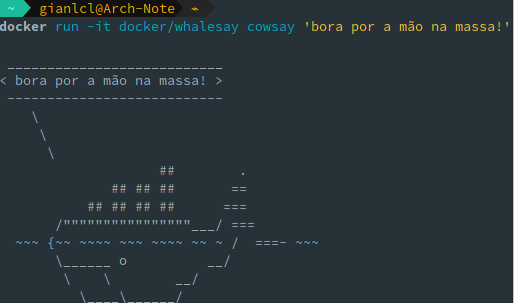
\includegraphics[width=0.8\linewidth]{AAUgraphics/whalesay1.png}
    \end{block}
\end{frame}

%subsection{Docker Images}
%\begin{frame}{Docker Images}{Primeiros Passos}
%    \begin{block}{O que é uma imagem?}
%    Uma imagem é um modelo no qual um container é baseado.
%    \end{block}
%\end{frame}
%
%\subsection{Inspect}
%\begin{frame}{Inspect}{Primeiros Passos}
%    \begin{block}{Inspect}
%    
%    \end{block}
%    \begin{itemize}
%        \item<1->
%    \end{itemize}
%\end{frame}

% \\\\\\\\\\\\\\\\\\\\\\\\\\\\\\\\\\\\\\\\\\\\\\\\\\\\\\\\
%  )||||||||||||||||||| AVANÇADO |||||||||||||||||||||||||)
% ////////////////////////////////////////////////////////
\section{Indo Além}

\subsection{Dockerfiles}
\begin{frame}{Criando Imagens}{Indo Além}
    \begin{block}{\textbf{Dockerfile}}
        Um \textit{Dockerfile} é como uma \textit{blueprint} de uma imagem, ele é um arquivo de texto com as instruções de passo a passo para a construção daquela imagem.\\
        O \textit{Dockerfile} é constituito por uma série de linhas com palavras-chaves com as quais você define os passo a passo da construção.\\[.5cm]
        \pause
        \centering
        \fcolorbox{lightgray}{softgray}{
            \minipage[t]{0.9\linewidth}
            \centering
                \textsc{palavras-chaves:}\\
                \textbf{\textsc{from, run, cmd, label, expose, env, add, copy, entrypoint, volume, user, workdir, arg, onbuild, stopsignal, healthcheck, shell}}
            \endminipage
        }\\[.5cm]
        \pause
        Após escrever o Dockefile basta rodar \texttt{\$ docker image build \textit{"caminho\_para\_Dockerfile"}} para construir a imagem.
    \end{block}
\end{frame}
\begin{frame}{Criando Imagens}{Indo Além}
    \begin{block}{\textbf{Camadas de uma Imagem}}
        \begin{itemize}
            \item<1-> Os containers do Docker funcionam baseado em camadas, essas camadas são pequenas imagens que juntas constituem uma docker image.
            \item<1-> Ao criar uma imagem de um container, o Docker compila cada parte do sistema numa camada e cria uma subimagem para cada camada.
            \item<1-> Dessa forma ele consegue reaproveitar essas subimagens para a criação de uma nova imagem que tenha camadas em comum com outra imagem já existente.
        \end{itemize}
    \end{block}
\end{frame}
\begin{frame}{Criando Imagens}{Indo Além}
    \centering
    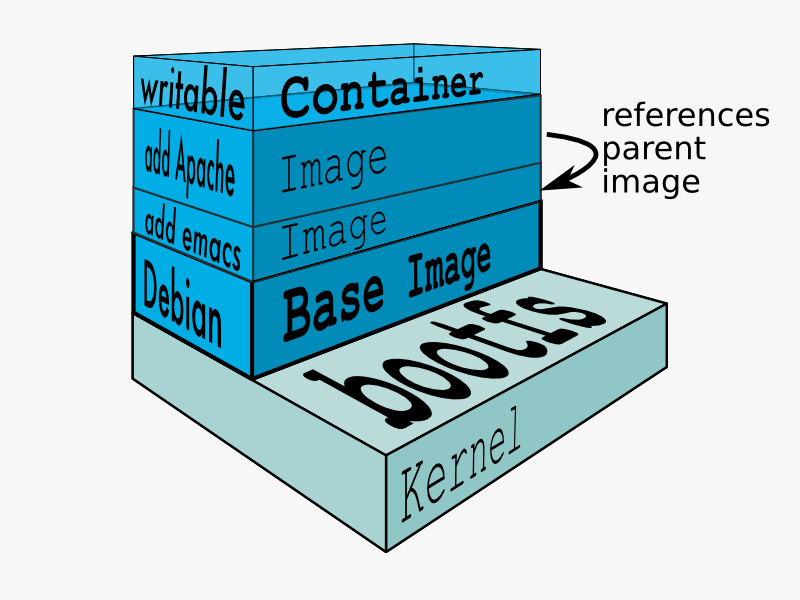
\includegraphics[width=0.8\linewidth]{AAUgraphics/docker_layers.png}
\end{frame}
\begin{frame}{Criando Imagens}{Indo Além}
    \centering
    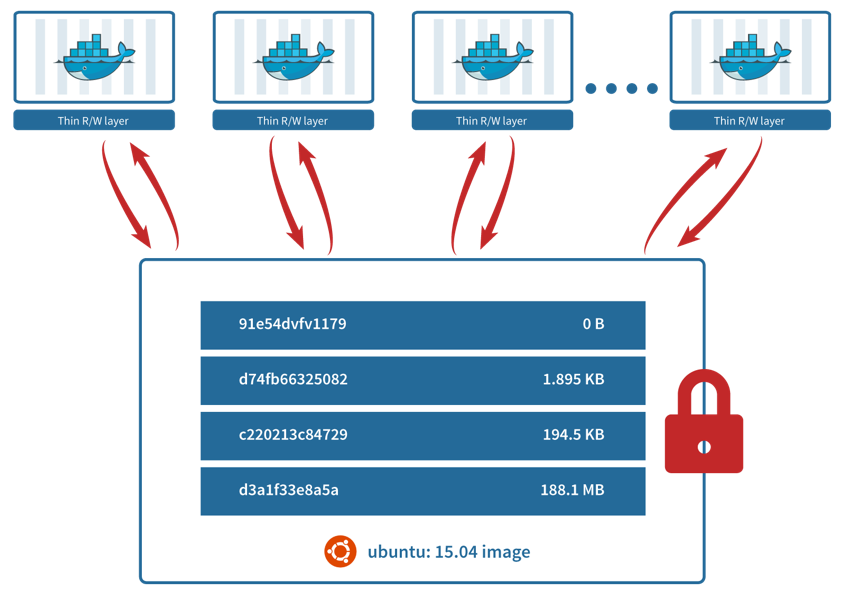
\includegraphics[width=0.8\linewidth]{AAUgraphics/docker-hash.png}
\end{frame}

\subsection{Conectando Aprendizados}
\begin{frame}{Conectando Aprendizados}{Indo Além}
    \begin{block}{\textbf{Criando stacks}}
    Um stack é um cluster de containers que trabalham em conjunto para formar uma aplicação.\\
    Existem duas formas de se criar uma stack.\\[.5cm]
    \end{block}
    \pause
    \begin{columns}
    \begin{column}{0.5\textwidth}
        \centering
        \textbf{Docker Compose}\\
        
\includegraphics[width=0.5\textwidth]{AAUgraphics/docker_compose.png}
        \pause
    \end{column}
    \begin{column}{0.5\textwidth}  %%<--- here
        \centering
        \textbf{Docker Stack}\\
        
\includegraphics[width=0.6\textwidth]{AAUgraphics/docker_stack.png}
    \end{column}
    \end{columns}
\end{frame}
%\begin{frame}{Conectando Aprendizados}{Indo Além}
%    \begin{block}{\textbf{Criando um Yaml}}
%    \end{block}
%\end{frame}

% \\\\\\\\\\\\\\\\\\\\\\\\\\\\\\\\\\\\\\\\\\\\\\\\\\\\\\\\
%  )||||||||||||||||||||||| FIM ||||||||||||||||||||||||||)
% ////////////////////////////////////////////////////////
{
\aauwavesbg%
    \begin{frame}[plain,noframenumbering]%
        \finalpage{
            \texttt{
                {\Huge
                Fim!
                }\\
                \vspace{0.2cm}
                pratique sem medo\\
                \href{https://labs.play-with-docker.com}
                    {labs.play-with-docker.com}
        }
    }
    \end{frame}
}

% \\\\\\\\\\\\\\\\\\\\\\\\\\\\\\\\\\\\\\\\\\\\\\\\\\\\\\\\
%  )|||||||||||||| FIM DO DOCUMENTO ||||||||||||||||||||||)
% ////////////////////////////////////////////////////////
\end{document}
